% vim: set foldmethod=marker foldlevel=0:

\documentclass[a4paper]{article}
\usepackage[UKenglish]{babel}

% NOTE: hyperref has to come before preamble
\usepackage[hidelinks]{hyperref}

\usepackage{preamble}

\usepackage{graphicx}
\graphicspath{ {./imgs/} }

\fancyhead[L]{MA265 Assignment 1}
\title{MA265 Methods of Mathematical Modelling 3, Assignment 1}
\colorlet{questionbodycolor}{green!50!teal!50}

\begin{document}

\maketitle

\setlength{\parindent}{0em}
\setlength{\parskip}{1em}

% {{{ Q1
\question{1}

\begin{questionbody}
\textit{Characterisation of second order PDEs}: State the types of the following equations:
\begin{enumerate}[(a)]
\item $u_{tt} - 4 u_{xx} = 0$
\item $u_t = 8 u_{xx}$
\item $u_{xx} + u_{yy} = 0$
\end{enumerate}
\end{questionbody}

% We use \@ before the full stop here because of the way LaTeX deals with interword and intersentence spacing in English. See https://tex.stackexchange.com/a/55112

\subsection{~} % 1.a

Linear, second order, hyperbolic, homogeneous PDE\@.

\subsection{~} % 1.b

Linear, second order, parabolic, homogeneous PDE\@.

\subsection{~} % 1.c

Linear, second order, elliptic, homogeneous PDE\@.

% }}}

% {{{ Q2
\newquestion{2}

\begin{questionbody}
\textit{The fundamental solution to the heat equation}: Verify that the solution to the heat equation \begin{equation}
u_t = k u_{xx} \quad x \in \R, t > 0
\label{eqn:heat-equation}
\end{equation}
for $k > 0$ is given by \[
u(x, t) = \f1{\sqrt{4 \pi kt}} \, \e^{-\f{x^2}{4 kt}}.
\] Set $k = 0.5$ and sketch $u$ at different times. What happens as $t \to 0$?
\end{questionbody}

We will differentiate the $u$ given in the question.
\begin{align*}
u &= {(4\pi kt)}^{-\f12} \e^{-x^2 {(4kt)}^{-1}} \\[1.5ex]
%
\partial_t u &= {(4\pi kt)}^{-\f12} \l( x^2 {(4k t^2)}^{-1} \e^{-x^2 {(4kt)}^{-1}} \r)
    - \f12 {(4\pi k t^3)}^{-\f12} \e^{-x^2 {(4kt)}^{-1}} \\[0.5ex]
&= {(4\pi kt)}^{-\f12} \e^{-x^2 {(4kt)}^{-1}} \l(
    x^2 {(4k t^2)}^{-1} - \f1{2t}
\r) \\[1.5ex]
%
\partial_x u &= {(4\pi kt)}^{-\f12} \l( -2x {(4kt)}^{-1} \r) \e^{-x^2 {(4kt)}^{-1}} \\[0.5ex]
&= -2x {(4\pi kt)}^{-\f12} {(4kt)}^{-1} \e^{-x^2 {(4kt)}^{-1}} \\[1.5ex]
%
\partial_{xx} u &= \partial_x \l( -2x {(4\pi kt)}^{-\f12} {(4kt)}^{-1} \e^{-x^2 {(4kt)}^{-1}} \r) \\[0.5ex]
&= -2 {(4\pi kt)}^{-\f12} {(4kt)}^{-1} \partial_x \l( x \e^{-x^2 {(4kt)}^{-1}} \r) \\[0.5ex]
&= -2 {(4\pi kt)}^{-\f12} {(4kt)}^{-1} \l(
    x \l( -2x {(4kt)}^{-1} \r) \e^{-x^2 {(4kt)}^{-1}}
    + \e^{-x^2 {(4kt)}^{-1}}
\r) \\[0.5ex]
&= -2 {(4\pi kt)}^{-\f12} {(4kt)}^{-1} \e^{-x^2 {(4kt)}^{-1}} \l( -2x^2 {(4kt)}^{-1} + 1 \r) \\[0.5ex]
&= 4 {(4\pi kt)}^{-\f12} {(4kt)}^{-1} \e^{-x^2 {(4kt)}^{-1}} \l( x^2 {(4kt)}^{-1} - \f12 \r)
\end{align*}

We want to have $\partial_t u = k \partial_{xx} u$, so let's look at each side and manipulate them to see if they're equal.
\begin{align*}
\partial_t u &= {(4\pi kt)}^{-\f12} \e^{-x^2 {(4kt)}^{-1}} \l(
    x^2 {(4k t^2)}^{-1} - \f1{2t}
\r) \\[0.5ex]
&= {(4\pi kt)}^{-\f12} \e^{-x^2 {(4kt)}^{-1}} \l(
    \f{x^2}{4k t^2} - \f1{2t}
\r) \\[1.5ex]
%
k \partial_{xx} u &= k {(4\pi kt)}^{-\f12} \e^{-x^2 {(4kt)}^{-1}} 4 {(4kt)}^{-1} \l(
    x^2 {(4kt)}^{-1} - \f12
\r) \\[0.5ex]
&= {(4\pi kt)}^{-\f12} \e^{-x^2 {(4kt)}^{-1}} \f{4k}{4kt} \l(
    \f{x^2}{4kt} - \f12
\r) \\[0.5ex]
&= {(4\pi kt)}^{-\f12} \e^{-x^2 {(4kt)}^{-1}} \l(
    \f{x^2}{4kt^2} - \f1{2t}
\r)
\end{align*}
Therefore this $u$ satisfies~\eqref{eqn:heat-equation}.

\begin{figure}[h]
    \centering
    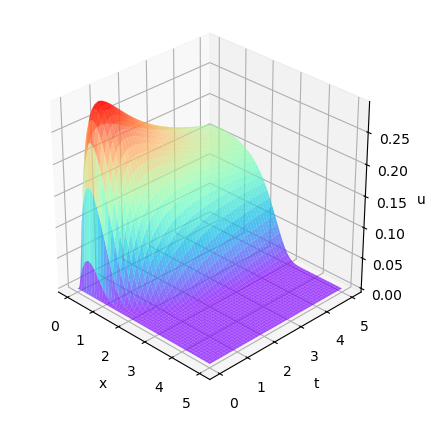
\includegraphics[scale=0.8]{Q2}
    \caption{A plot of $u(x, t)$ with $k=0.5$}
\end{figure}

As $t \to 0$, the model breaks down.

% }}}

% {{{ Q3
\newquestion{3}

\begin{questionbody}
\textit{Well-posedness}: Consider the elliptic problem \begin{align*}
u_{xx}(x) &= f(x) \qquad\qquad x \in [0, 1] \tag{\dagger}\label{eqn:Q3-elliptic-system} \\
u_x(0) &= u_x(1) = 0
\end{align*}

Let $u^*$ denote a solution to~\eqref{eqn:Q3-elliptic-system}.
\begin{enumerate}[(a)]
\item Are there any other solutions to~\eqref{eqn:Q3-elliptic-system}? If yes, state them.
\item Show that \[ \intlim 0 1 {f(x)} x = 0 \] is a necessary condition to have a solution. \textbf{Hint}: Integrate~\eqref{eqn:Q3-elliptic-system} and use the boundary conditions.
\end{enumerate}
\end{questionbody}

\subsection{~} % 3.a

Yes. Any function $v(x) = u^*(x) + C$, where $C \ne 0$ is any constant, is also a solution to~\eqref{eqn:Q3-elliptic-system}.

\subsection{~} % 3.b

We integrate both sides of~\eqref{eqn:Q3-elliptic-system} and get \begin{align*}
\intlim 01 {u_{xx}} x &= \intlim 01 {f(x)} x \\
u_x(1) - u_x(0) &= \intlim 01 {f(x)} x \\
0 &= \intlim 01 {f(x)} x
\end{align*}

% }}}

% {{{ Q4
\newquestion{4}

\begin{questionbody}
\textit{Method of characteristics}: Use the method of characteristics to solve the transport equation \[
u_t + v(x, t) u_x = 0
\] in $\R \times (0, \infty)$ with initial condition $u(x, 0) = \Phi_0(x) = 1 - 2x$ for the velocity field \[
v(x, t) = \f{1 + t^2}2.
\]
\end{questionbody}

We first have to solve the associated ODE to use the method characteristics.
\begin{align*}
\xi'(t) &= v(\xi(t), t) = \f{1 + t^2}2 \\
\xi(0) &= x_0
\end{align*}

We can solve this with separation of variables.
\begin{align*}
\dd \xi t &= \f{1 + t^2}2 \\[0.5ex]
\inte {} \xi &= \f12 \inte {1 + t^2} t \\[0.5ex]
\xi(t) &= \f12 t + \f16 t^3 + C
% \xi(0) &= 0 + 0 + C = x_0
\end{align*}

We use the initial value to find that \[ \xi(t) = \f12 t + \f16 t^3 + x_0. \]

% Then $x = \xi(t)$ equals something with $x_0$, so solve for $x_0$ in terms of $x$ and $t$. Then $u(x, t) = \Phi_0(x_0)$, which should contain both $x$ and $t$.

We know that $x = \xi(t)$, so we can solve for $x_0$ and find that \[ x_0 = x - \f12 t - \f16 t^3. \]

Now we apply the fact that $u(x, t) = \Phi_0(x_0)$ to find that
\begin{align*}
u(x, t) &= 1 - 2x_0 \\
&= 1 - 2 \l( x - \f12 t - \f16 t^3 \r) \\
&= 1 - 2x + t + \f13 t^3.
\end{align*}

% }}}

% {{{ Q5
\newquestion{5}

\begin{questionbody}
\textit{Classification of PDEs}: Reduce the elliptic equation \[
u_{xx} + 3 u_{yy} - 2 u_x + 24 u_y + 5u = 0
\] to the equation \[
v_{xx} + v_{y' y'} + cv = 0
\] by changing the dependant variable to $u(x, y) = v(x, y) \e^{\alpha x + \beta y}$ and then using the scaling $y' = \gamma y$. What are the values of $\alpha$, $\beta$, $\gamma$, and $c$?
\end{questionbody}

We will begin by calculating the derivatives of $u$.
\begin{align*}
u(x, y) &= v(x, y) \e^{\alpha x + \beta y} \\[1.5ex]
%
u_x &= \alpha v \e^{\alpha x + \beta y} + v_x \e^{\alpha x + \beta y} \\[0.5ex]
&= \e^{\alpha x + \beta y} \l( \alpha v + v_x \r) \\[1.5ex]
%
u_{xx} &= \e^{\alpha x + \beta y} \l( \alpha v_x + v_{xx} \r) + \alpha \e^{\alpha x + \beta y} \l( \alpha v + v_x \r) \\[0.5ex]
&= \e^{\alpha x + \beta y} \l( v_{xx} + 2\alpha v_x + \alpha^2 v \r) \\[1.5ex]
%
u_y &= \e^{\alpha x + \beta y} \l( \beta v + v_y \r) \\[1.5ex]
%
u_{yy} &= \e^{\alpha x + \beta y} \l( v_{yy} + 2\beta v_y + \beta^2 v \r)
\end{align*}

We plug these into the equation and get \[ \begin{split}
0 &= u_{xx} + 3 u_{yy} - 2 u_x + 24 u_y + 5u \\[1.5ex]
&= \e^{\alpha x + \beta y} \Big(
    v_{xx} + 2\alpha v_x + \alpha^2 v \\
    &\quad + 3 \l( v_{yy} + 2\beta v_y + \beta^2 v \r) \\
    &\quad - 2 \l( \alpha v + v_x \r) \\
    &\quad + 24 \l( \beta v + v_y \r) \\
    &\quad + 5v
\Big) \\[1.5ex]
&= \e^{\alpha x + \beta y} \Big(
    v_{xx} + 2 \alpha v_x + \alpha^2 v \\
    &\quad + 3 v_{yy} + 6 \beta v_y + 3 \beta^2 v \\
    &\quad - 2 \alpha v - 2 v_x \\
    &\quad + 24 \beta v + 24 v_y \\
    &\quad + 5v
\Big) \\[1.5ex]
&= \e^{\alpha x + \beta y} \Big(
    v_{xx} + 3 v_{yy} \\
    &\quad + \l( 2\alpha - 2 \r) v_x + \l( 6\beta + 24 \r) v_y \\
    &\quad + \l( \alpha^2 + 3\beta^2 - 2\alpha + 24\beta + 5 \r) v
\Big)
\end{split} \]

The coefficients of $v_x$ and $v_y$ are 0, so we need $2\alpha - 2 = 0$ and $6\beta + 24 = 0$, which implies $\alpha = 1$ and $\beta = -4$. Therefore the equation becomes
\begin{align*}
0 &= \e^{x - 4y} \l(
    v_{xx} + 3 v_{yy}
    + \l( 1 + 12 - 2 - 96 + 5 \r) v
\r) \\[0.5ex]
&= \e^{x - 4y} \l(
    v_{xx} + 3 v_{yy}
    - 78 v
\r) \\[0.5ex]
\implies 0 &= v_{xx} + 3 v_{yy} - 78 v
\end{align*}

We can divide out the $\e^{x - 4y}$ because it is never 0. We can also observe that if $y' = \gamma y$, then $\gamma^2 v_{y' y'} = v_{yy}$ so $v_{y' y'} = \f1{\gamma^2} v_{yy}$.

Then we conclude that $\alpha = 1$, $\beta = -4$, $\gamma = \f1{\sqrt3}$, $c = -78$.

% }}}

\end{document}
